\documentclass[a4paper,11pt]{article}
\usepackage{filecontents}

\usepackage[utf8]{inputenc}
\usepackage[english]{babel}
\usepackage{graphicx, array, blindtext}
\usepackage[colorinlistoftodos]{todonotes}
\DeclareUnicodeCharacter{2212}{-}
\usepackage [a4 paper , hmargin = 1.2 in , bottom = 1.5 in] {geometry}
\usepackage [parfill] {parskip}

\usepackage{enumitem}
\usepackage{amsmath}
\usepackage{amsthm}

\usepackage{nameref}
\usepackage{amssymb}
\usepackage [linesnumbered, ruled, vlined] {algorithm2e}
\usepackage{listings}
\usepackage{xcolor}
\usepackage{floatrow}
\usepackage{siunitx}


\usepackage{cancel}
\usepackage{fancyhdr}
\usepackage{graphicx}
\usepackage{verbatim}
\usepackage[document]{ragged2e}

\renewcommand{\footrulewidth}{0.4pt}
\newtheorem{definition}{Definition}
\numberwithin{definition}{section}
\newtheorem{mytheorem}{Theorem}
\numberwithin{mytheorem}{subsection}
\newcommand{\notimplies}{\;\not\!\!\!\longrightarrow}  
\newcommand\norm[1]{\left\lVert#1\right\rVert}
\pagestyle{fancy}
\fancyhf{}
\rhead{CS754 Assignment 1}
\lhead{200050013-200050130}
\fancyfoot[C]{Page \thepage}
\usepackage{subcaption}
\usepackage{listings}


\usepackage{hyperref}
\urlstyle{same}
\hypersetup{pdftitle={main.pdf},
    colorlinks=false,
    linkbordercolor=red
}
\usepackage{array}
\usepackage{listings,chngcntr}

\begin{document}
\centering{

\title{\fontsize{150}{60}{CS754 Assignment 1 Report}}

\author{
Arpon Basu \\ Shashwat Garg }
}

\date{Spring 2022}
\maketitle

\justifying
\tableofcontents

\newpage
\justifying
\section*{Introduction}

Welcome  to our report on CS754 Assignment 1. We have tried to make this report comprehensive and self-contained. We hope reading this would give you a proper flowing description of our work, methods used and the results obtained. Feel free to keep our code scripts alongside to know the exact implementation of our tasks. 

We have referred to some sites on the web for finding the MATLAB implementations (generic documentation pages) and the same has been added in the references section. 

In many places, to better give context to the place from which the questions could have arisen, some theoretical discussions have been engaged in.

Hope you enjoy reading the report. Here we go!




\newpage
\section{Problem 1}
We have been given the following problem-

Let $\boldsymbol{\theta^{\star}}$ : $\textrm{min} \|\boldsymbol{\theta}\|_1$ such that $\|\boldsymbol{y}-\boldsymbol{\Phi \Psi \theta}\|_2 \leq \varepsilon$, where $\boldsymbol{x} = \boldsymbol{\Psi \theta}$ and $\boldsymbol{y} = \boldsymbol{\Phi x} + \boldsymbol{\eta}$. $\varepsilon$ is an upper bound on the magnitude of the noise vector $\boldsymbol{\eta}$.

Also, Theorem 3 states-\\If $\boldsymbol{\Phi}$ obeys the restricted isometry property with isometry constant $\delta_{2s} < \sqrt{2}-1$, then we have $\|\boldsymbol{\theta} - \boldsymbol{\theta^{\star}}\|_2 \leq C_1 s^{-1/2}\|\boldsymbol{\theta}-\boldsymbol{\theta_s}\|_1 + C_2 \varepsilon$ where $C_1$ and $C_2$ are functions of only $\delta_{2s}$ and where $\forall i \in \mathcal{S}, \boldsymbol{\theta_s}_i = \theta_i; \forall i \notin \mathcal{S}, \boldsymbol{\theta_s}_i = 0$.

\subsection{Trend of Error Bound with $s$}
This is not a discrepancy. In reality, we are ignoring the change in $C_1$ and $C_2$. The point is, we are only focusing on the effect of $s^{-1/2}$ and $||\boldsymbol{\theta}-\boldsymbol{\theta_s}||_1$. We must also see the changes in $C_1$ and $C_2$, which increase as the value of $\delta_{2s}$ changes.

As the value of $s$ increases, due to reducing sparsity, we observe that (the bound on) $\delta_{2s}$ also increases. Intuitively, this is because an increase in $s$ implies an increase in the required number of linearly independent columns required in the $\boldsymbol{\Phi \Psi}$ matrix. This is unlikely as s increases. An increase in $\delta_{2s}$ leads to an increase in the value of $C_1$ and $C_2$.

Thus we have two opposing behaviours and we cannot claim that the error bound improves as the sparsity measure, $s$ increases in value.

\subsection{Dependence of error bound on $m$}

$m$ does not directly affect the error bound but it has several other indirect implications. 

First of all, we require our matrix $\boldsymbol{A}=\boldsymbol{\Phi \Psi}$ to obey the RIP, for which we usually construct our sensing matrix $\boldsymbol{\Phi}$ using Gaussian or Bernoulli entries randomly. The probablility that this happens is very high in case $m \geq CS log(n/S)$.

Apart from this, $m$ also affects the value of $\epsilon$ which we can take in case of uniform Gaussian noise in the measurements. In such cases, a good approximation of $\epsilon$ is given by 3 standard deviations around the mean, which effectively transaltes into $\epsilon \geq 9m\sigma^2$.

Finally, when $m$ increases, we observe that the rank of the matrix $\boldsymbol{A}$ increases, which would make it satisfy the RIP with a higher probablility. This would indicate a drop in the value of $\delta_{2s}$, indicating a drop in the constants $C1$ and $C2$ and thus improving the error bound.

Thus, m has a lot of indirect implications in the error bound.

\subsection{Change in requirement of $\delta_{2s}$}

Theorem 3 is better than Theorem 3A. Theorem 3 provides the same guarantees for more relaxed values of $\delta_{2s}$.

For large $\delta_{2s}$ we can work with comparatively less sparse signals. For values of $\delta_{2s} \geq 0.1$, Theorem 3A doesn't guarantee anything while the Theorem 3 works well for all values till 0.4142.

Also, for values of $\delta_{2s} \leq 0.1$, both the theorems give the exact same reconstructions.

Thus, Theorem 3 is much more useful.


\subsection{Setting $\epsilon = 0$}

This is not the correct way to solve the problem in presence of noise.

By setting the $\epsilon$ to 0, we have ignored the noise and thus our $\theta$ obtained from such a method will be incorrect. We might encounter several problems. We might not be able to converge on a value, because a solution does not even exist in this case of constraints. We might overfit our measurements to include noise which would result in the $\theta$ not being the sparsest and correct measurement.

Instead, we should choose an $\epsilon$ greater than the noise magnitude, for good results.



\newpage


\section{Problem 2}
We note that this problem has two parts: One for demonstrating that the upper bound of $\mu(\boldsymbol{\Phi, \Psi})$ is $\sqrt{n}$, and one for demonstrating that the lower bound of $\mu(\boldsymbol{\Phi, \Psi})$ is 1. We shall deal with both parts separately.\\
\subsection{Lower Bound}
\begin{proof}
Since $\boldsymbol{\Psi}$ is an orthonormal matrix, it's column vectors $\boldsymbol{\Psi_1}$, $\boldsymbol{\Psi_2}$, ..., $\boldsymbol{\Psi_n}$ form a orthonormal basis for $\mathbb{K}^n$, and consequently we can express $\boldsymbol{g}$ as $\sum_{k=1}^{n} \alpha_k\boldsymbol{\Psi_k}$. Also, $\lVert \boldsymbol{g}\rVert_2 = \sqrt{\sum_{j=1}^{n} \alpha^2_j}$, following which we get $\boldsymbol{g}_{\mathrm{normalized}} = \sum_{k=1}^{n} \frac{\alpha_k}{\sqrt{\sum_{j=1}^{n} \alpha^2_j}}\boldsymbol{\Psi_k}$. Thus $\mu(\boldsymbol{g, \Psi)} = \sqrt{n}\cdot\mathrm{max}_{i\in[n]}\;|\boldsymbol{g}_{\mathrm{normalized}}^T\boldsymbol{\Psi_i}| = \sqrt{n}\cdot\mathrm{max}_{i\in[n]}\;\frac{|\alpha_i|}{\sqrt{\sum_{j=1}^{n} \alpha^2_j}}$. WLOG assuming that $|\alpha_1| = \mathrm{max}_{i\in[n]}\;|\alpha_i|$, we get that
$$\mu(\boldsymbol{g, \Psi}) \geq \sqrt{n}\cdot\mathrm{max}_{i\in[n]}\;\frac{|\alpha_i|}{\sqrt{\sum_{j=1}^{n} |\alpha_1|^2}} = \sqrt{n}\frac{|\alpha_1|}{\sqrt{n\alpha^2_1}} = 1$$
as desired. Note that equality is achieved iff $\alpha_1 = \alpha_2 = ... = \alpha_n$.
\end{proof}
\subsection{Upper Bound}
\begin{proof}
Directly borrowing from the previous proof, $\mu(\boldsymbol{g, \Psi)} = \sqrt{n}\cdot\mathrm{max}_{i\in[n]}\;|\boldsymbol{g}_{\mathrm{normalized}}^T\boldsymbol{\Psi_i}|$. Now, by the Cauchy Schwartz inequality, for any two vectors $\mathbf{u}$, $\mathbf{v}$, we have $|\langle \mathbf{u}, \mathbf{v}\rangle|\leq \lVert \mathbf{u}\rVert_2\lVert \mathbf{v}\rVert_2$, where $|\langle \cdot, \cdot\rangle|$ is the usual Euclidean inner product. Applying it to the coherence relation yields $|\boldsymbol{g}_{\mathrm{normalized}}^T\boldsymbol{\Psi_i}| \leq \lVert \boldsymbol{g}_{\mathrm{normalized}}\rVert_2\lVert \boldsymbol{\Psi_i}\rVert_2 = 1$, and consequently we obtain that $\mu(\boldsymbol{g, \Psi)} \leq \sqrt{n}$, as desired. Note that equality is achieved iff $\boldsymbol{g}$ is parallel to some column vector $\boldsymbol{\Psi_i}$ of $\boldsymbol{\Psi}$.
\end{proof}

\newpage
\section{Problem 3}

This is a problem based on the basic concepts of linear algebra and the concepts of basis vectors, null-space property and independent vectors.

We have a compressed measurement $y$, of the form $\mathbf{y} = \mathbf{\Phi x}$ where $\mathbf{\Phi} \in \mathbb{R}^{m \times n}$ is the measurement matrix and $\mathbf{x} \in \mathbb{R}^n, ~n \gg 2$. Consequently, $\mathbf{y} \in \mathbb{R}^m ~(m \ll n$). Our aim is to figure out $\mathbf{x}$

\subsection{m=1}
Now observe that $\mathbf{\Phi}$ is essentially a row vector and $\mathbf{x}$ is a column vector, thus, even if only a element of x was non-zero, we still do not know which index of $\mathbf{\Phi}$ and $\mathbf{x}$ combine to give the value of $\mathbf{y}$, which is effectively a scalar in this case.

On the other hand, if we know the value of index, then the vector $\mathbf{x}$ is deducible. If the index is $i$, then the elements of $\mathbf{x}$ are zero for all indices $j\neq i$ and equal to $\mathbf{y/\Phi_i}$ for the $i^{th}$ index.

Thus, answer of the first part is NO, and the second part is YES.

\subsection{m=1}

Yes! It is possible in this case, if $\mathbf{x}$ has only one non-zero element.

Since $\mathbf{x}$ has only one non-zero entry, say index $i$, only a single column of $\mathbf{\Phi}$ plays a role in getting the value of $\mathbf{y}$.

Thus, effectively,
$$\mathbf{y^1} = \mathbf{\Phi_i^1.x^i}$$
$$\mathbf{y^2} = \mathbf{\Phi_i^2.x^i}$$

This implies that the ratio of the values in the $\mathbf{y}$ vector, matches the ratio of the values in some column of the $\mathbf{\Phi}$ matrix.

If our $\mathbf{\Phi}$ matrix is sufficiently randomly generated, we can always uniquely find such an index.

After that, it is just like the previous question. If the index found is $i$, then the elements of $\mathbf{x}$ are zero for all indices $j\neq i$ and equal to $\mathbf{y^1/\Phi_i^1}$ or $\mathbf{y^2/\Phi_i^2}$ for the $i^{th}$ index.

Again, please note that the success of this method depends on the fact that all columns of $\mathbf{\Phi}$ are linearly independent, which is a valid assumption given the nature of $\mathbf{\Phi}$.

\subsection{m=3}

Here, we have a 2-sparse $\mathbf{x}$ vector and 3 measurements.
Effectively, we need to solve the following linear system-

$$\mathbf{y^1} = \mathbf{\Phi_i^1.x^i + \Phi_j^1.x^j}$$
$$\mathbf{y^2} = \mathbf{\Phi_i^2.x^i + \Phi_j^1.x^j}$$
$$\mathbf{y^3} = \mathbf{\Phi_i^3.x^i + \Phi_j^1.x^j}$$

Note that we do not have any idea about which indices the $i$ and $j$ might be.\\
Just as we looked at the ratio in the previous part, here we need to look at the span of the two column vectors $\mathbf{\Phi_i}$ and $\mathbf{\Phi_j}$. If the vector $\mathbf{y}$ lies in the span of the two vectors, then we can find an appropriate solution to the values of vector $\mathbf{x}$.

But there is a problem. Note that the choice of $i$ and $j$ is not unique. We know that the $m << n$. Thus, given that $\mathbf{\Phi_i}$ is a random matrix, there is a high chance that we can choose another set of 2 vectors with indices $k$ and $l$ such that $\mathbf{y}$ lies in the span of $\mathbf{\Phi_k}$ and $\mathbf{\Phi_l}$.

In fact, given a large enough $n$, it is certain that there will exist 4 vectors (of dimension 3) which are linearly dependent and none of the coefficients
($\alpha_i,~\alpha_j,~\alpha_k,~\alpha_l$) is zero. This means that we will always have 2 ways of representing our $\mathbf{y}$ vector. This implies that, we cannot always get the $\mathbf{x}$ vector in this case.

Surprisingly, without knowing the indices at which x is non-zero, we cannot even generate a specific $\mathbf{\Phi}$ such that we would have the vector $\mathbf{x}$. This is because such a $\mathbf{\Phi}$ would require most of the columns to be zero in atleast 2 places out of 3, such that we cannot get 4 linearly dependent columns with all $\alpha_i,~\alpha_j,~\alpha_k,~\alpha_l$ as non-zero. This would ensure that there is always a unique pair of indices that calculate $\mathbf{y}$, but again, it is not possible in the current scenario.


\subsection{m=4}

This problem very closely resembles the null-space theorem covered in the lectures. We have a 2-sparse vector and a matrix with m=4. If we can ensure that any 4 columns are linearly independent then we have a solution. 

If you are wondering about whether we might fail due to 5 such columns being linearly dependent, note that in that case, we would have a 2 column representation equal to a 3 column representation. But a 3 column representation is useless in this case. Thus, we can avoid it.\footnote{The previous case, for m=3 fails because in that case, any 4 columns are linearly dependent. Thus, we can get a 2 column representation equal to another 2 column representation, which leads to multiple solutions.}

The solution is as follows-

We assume that the matrix is of rank=4. This implies that a unique solution exists. We follow the following algorithm.

\begin{itemize}
    \item Iterate over all pairs of columns in the matrix $\mathbf{\Phi}$
    \item Check if the vector $\mathbf{y}$ lies in the span of the two column vectors in focus.
\end{itemize}

As long as the rank=4, there exists only a single solution for the algorithm.
Otherwise, we have two 2-sparse vectors as solution. This implies that their difference ie. a 4-sparse vector lies in the null-space of $\mathbf{\Phi}$. This is a contradiction to our assumption. Hence proved.

Thus, the answer to this part is YES (mostly, since there is a certain randomness involved in creation of these matrices).


\newpage


\section{Problem 4}

We provide a short and sweet proof for this problem below.
\begin{proof}
We set up some notation first: Let 
\begin{gather*}
    \boldsymbol{x^*} :=  \mathrm{arg\;min}\boldsymbol{_{\lVert y - Ax\rVert_2 \leq e}\;\lVert x\rVert_1} \\
    \boldsymbol{l_1 := } \mathrm{min}\boldsymbol{_{\lVert y - Ax\rVert_2 \leq e}\;\lVert x\rVert_1} \\
    \boldsymbol{f(t) := } \mathrm{arg\;min}\boldsymbol{_{\lVert x\rVert_1 \leq t}\; \lVert y - Ax\rVert_2} 
\end{gather*}
Then note that if $\boldsymbol{t < l_1}$, $\boldsymbol{f(t) > e}$: Why? Because if $\boldsymbol{f(t) \leq e}$, then one would have that there exist $\boldsymbol{x}$ with L1-norm lesser than $\boldsymbol{l_1}$ which nevertheless make the L2 norm of $\boldsymbol{(y - Ax)}$ $\leq$ $\boldsymbol{e}$, which contradicts the minimality of $\boldsymbol{x^*}$.\\
Also note that $\boldsymbol{f(l_1) \leq e}$, since we have a witness $\boldsymbol{x^*}$ for which the L1-norm is equal to $\boldsymbol{l_1}$ and $\boldsymbol{\lVert y - Ax^*\rVert_2 \leq e}$ due to the premise of the problem P1. Thus it's clear that all minimizers of $\boldsymbol{\lVert y - Ax\rVert_2}$ under the conditions $\boldsymbol{\lVert x\rVert_1 \leq l_1}$ actually lie only on the ``sphere" $\boldsymbol{\lVert x\rVert_1 = l_1}$ (because for points strictly to the interior of this ``sphere", $\boldsymbol{\lVert y - Ax\rVert_2}$ assumes values larger than $\boldsymbol{e}$). Now, if it so happens that there exists another $\boldsymbol{z}$ (such that $\boldsymbol{\lVert z\rVert_1 = l_1}$) such that $\boldsymbol{\lVert y - Az\rVert_2 \leq e}$, then we note that the \emph{uniqueness} of $\boldsymbol{x^*}$ is violated, as $\boldsymbol{z}$ also becomes a minimizer for P1 (along with $\boldsymbol{x^*}$) since it satisfies the premise of P1 (which is $\boldsymbol{\lVert y - Ax\rVert_2 \leq e}$).\\
Thus, we have that for $\boldsymbol{t = \mathrm{min}_{\lVert y - Ax\rVert_2 \leq e}\;\lVert x\rVert_1}$, both the problems P1 and Q1 have the \textbf{same unique minimizer}.\\
Hence proved.
\end{proof}

\newpage
\section{Problem 5}

(a) The title of the paper we reviewed was \textbf{Low-Complexity FPGA Implementation of
Compressive Sensing Reconstruction}. It was published in \textbf{2013} by \textbf{IEEE} in the \textbf{International Conference on Computing, Networking and Communications, Multimedia Computing and Communications
Symposium}.\\
(b) The main aim of the paper is to optimize the hardware time required for executing reconstruction algorithms like \textbf{OMP}. To that end, it develops a novel hardware architecture which promises to deliver a execution time 3.4 $\times$ faster than what conventional hardware takes to execute OMP. The conceptualization and execution of the paper is best explained through the two images below.\\
\begin{figure}
    \begin{center}
        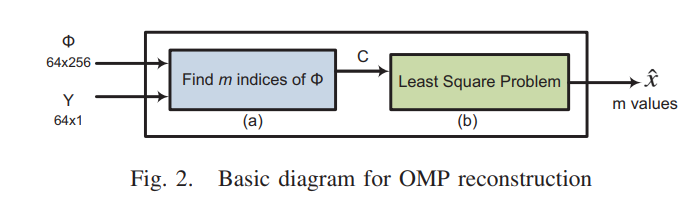
\includegraphics[scale=0.5]{Basic Structure of OMP.png}
        \caption{Basic Structure of OMP}
    \end{center}
\end{figure}

\begin{figure}
    \begin{center}
        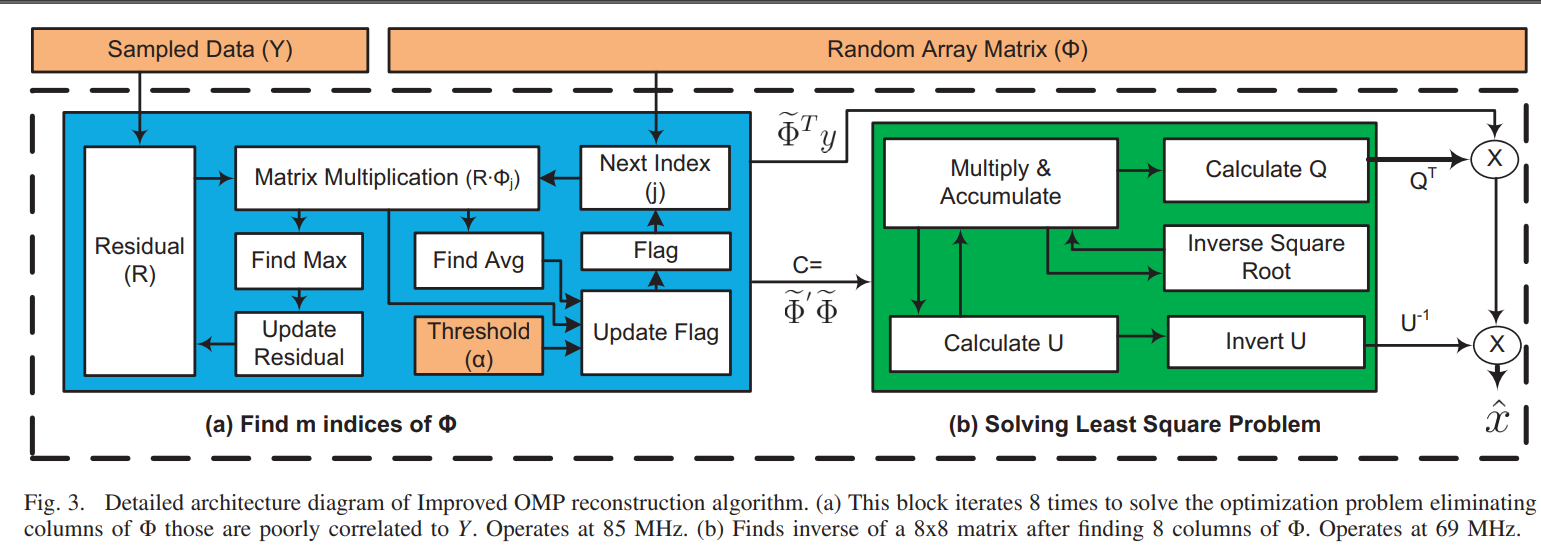
\includegraphics[scale=0.5]{Proposed HArdware Architecture.png}
        \caption{Proposed Hardware Architecture}
    \end{center}
\end{figure}
(c) This paper optimizes the execution of the \textbf{reconstruction technique OMP} which is very widely used in compressed sensing scenario. This paper per se itself doesn't deploy compressed sensing towards any goal but rather seeks to improve what already exists. 




\newpage

\section{Problem 6}












\end{document}



